\thispagestyle{lichsutoanhocnone}
\pagestyle{lichsutoanhoc}
\graphicspath{{../lichsutoanhoc/pic/}}
\everymath{\color{lichsutoanhoc}}
\blfootnote{$^1$\color{lichsutoanhoc}Cộng tác viên Viện Toán học.}
\begingroup
\AddToShipoutPicture*{\put(0,616){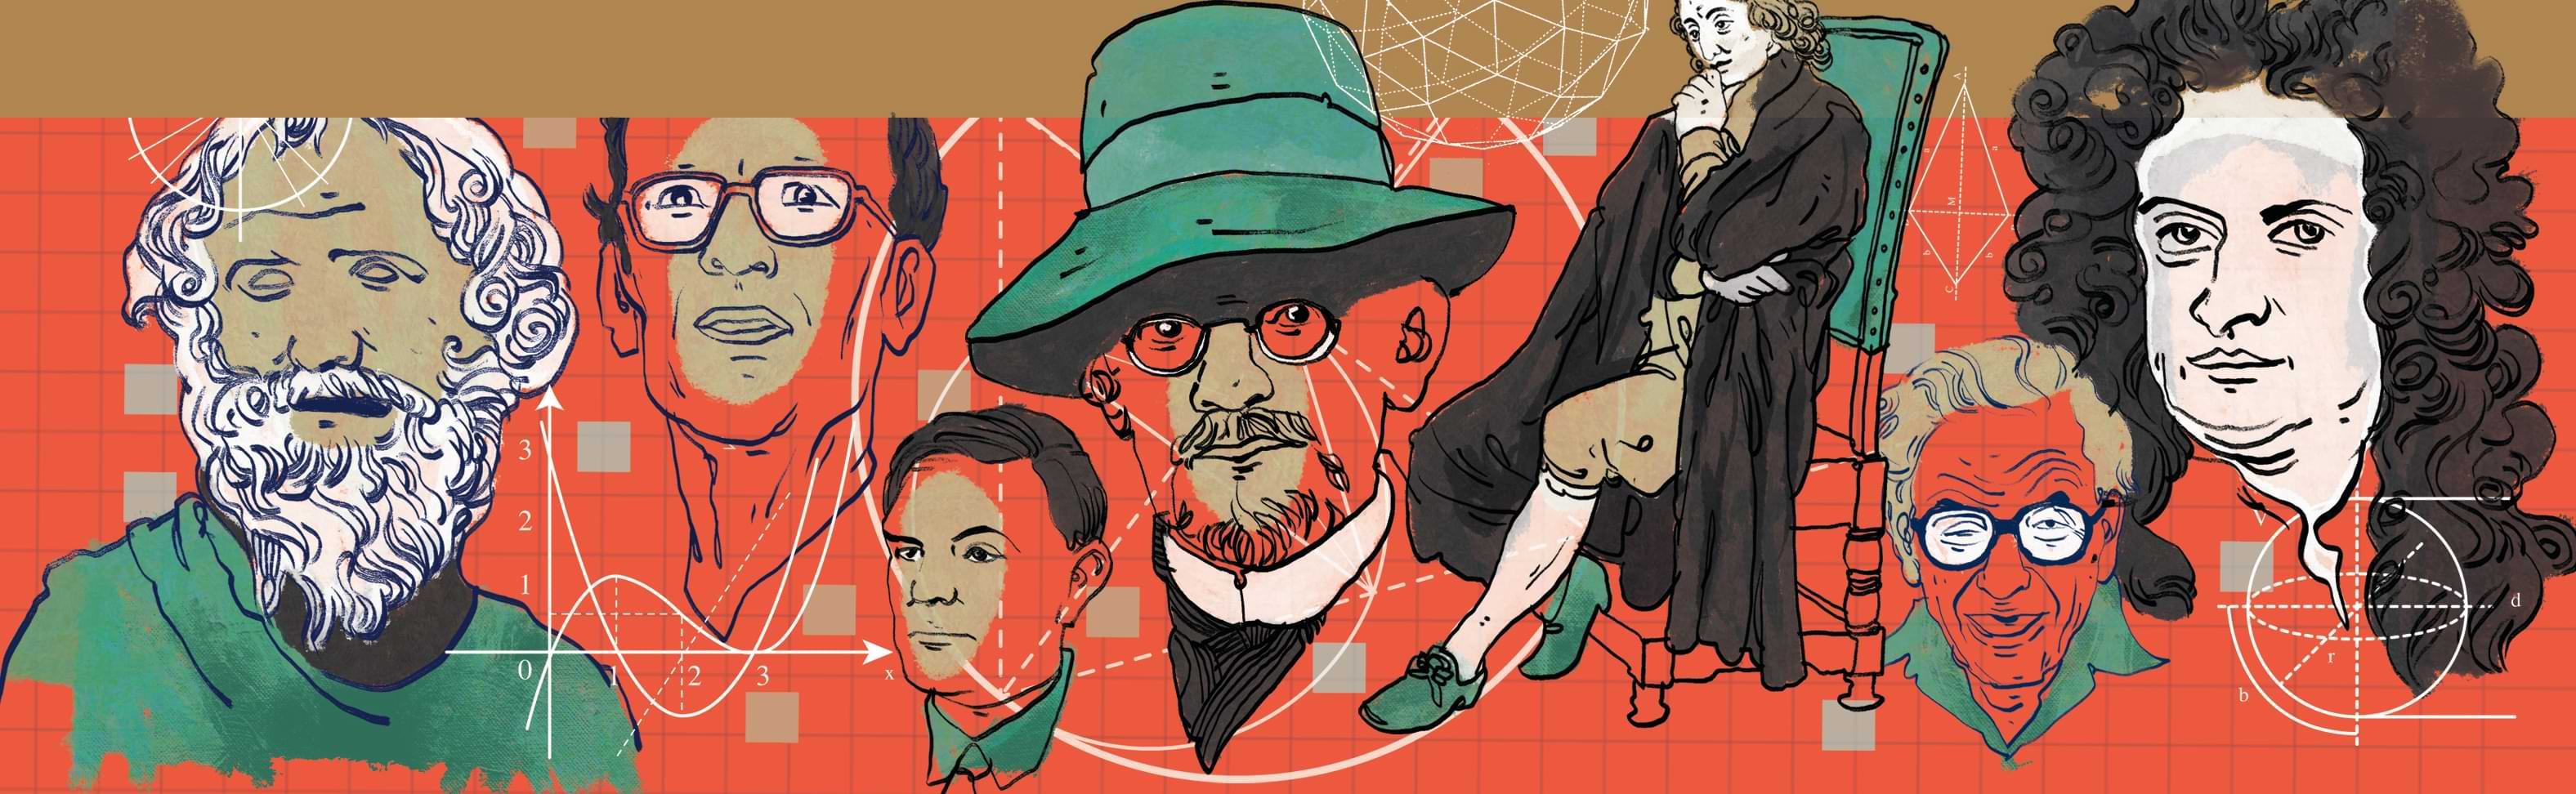
\includegraphics[width=19.3cm]{../bannerlichsu}}}
\AddToShipoutPicture*{\put(104,525){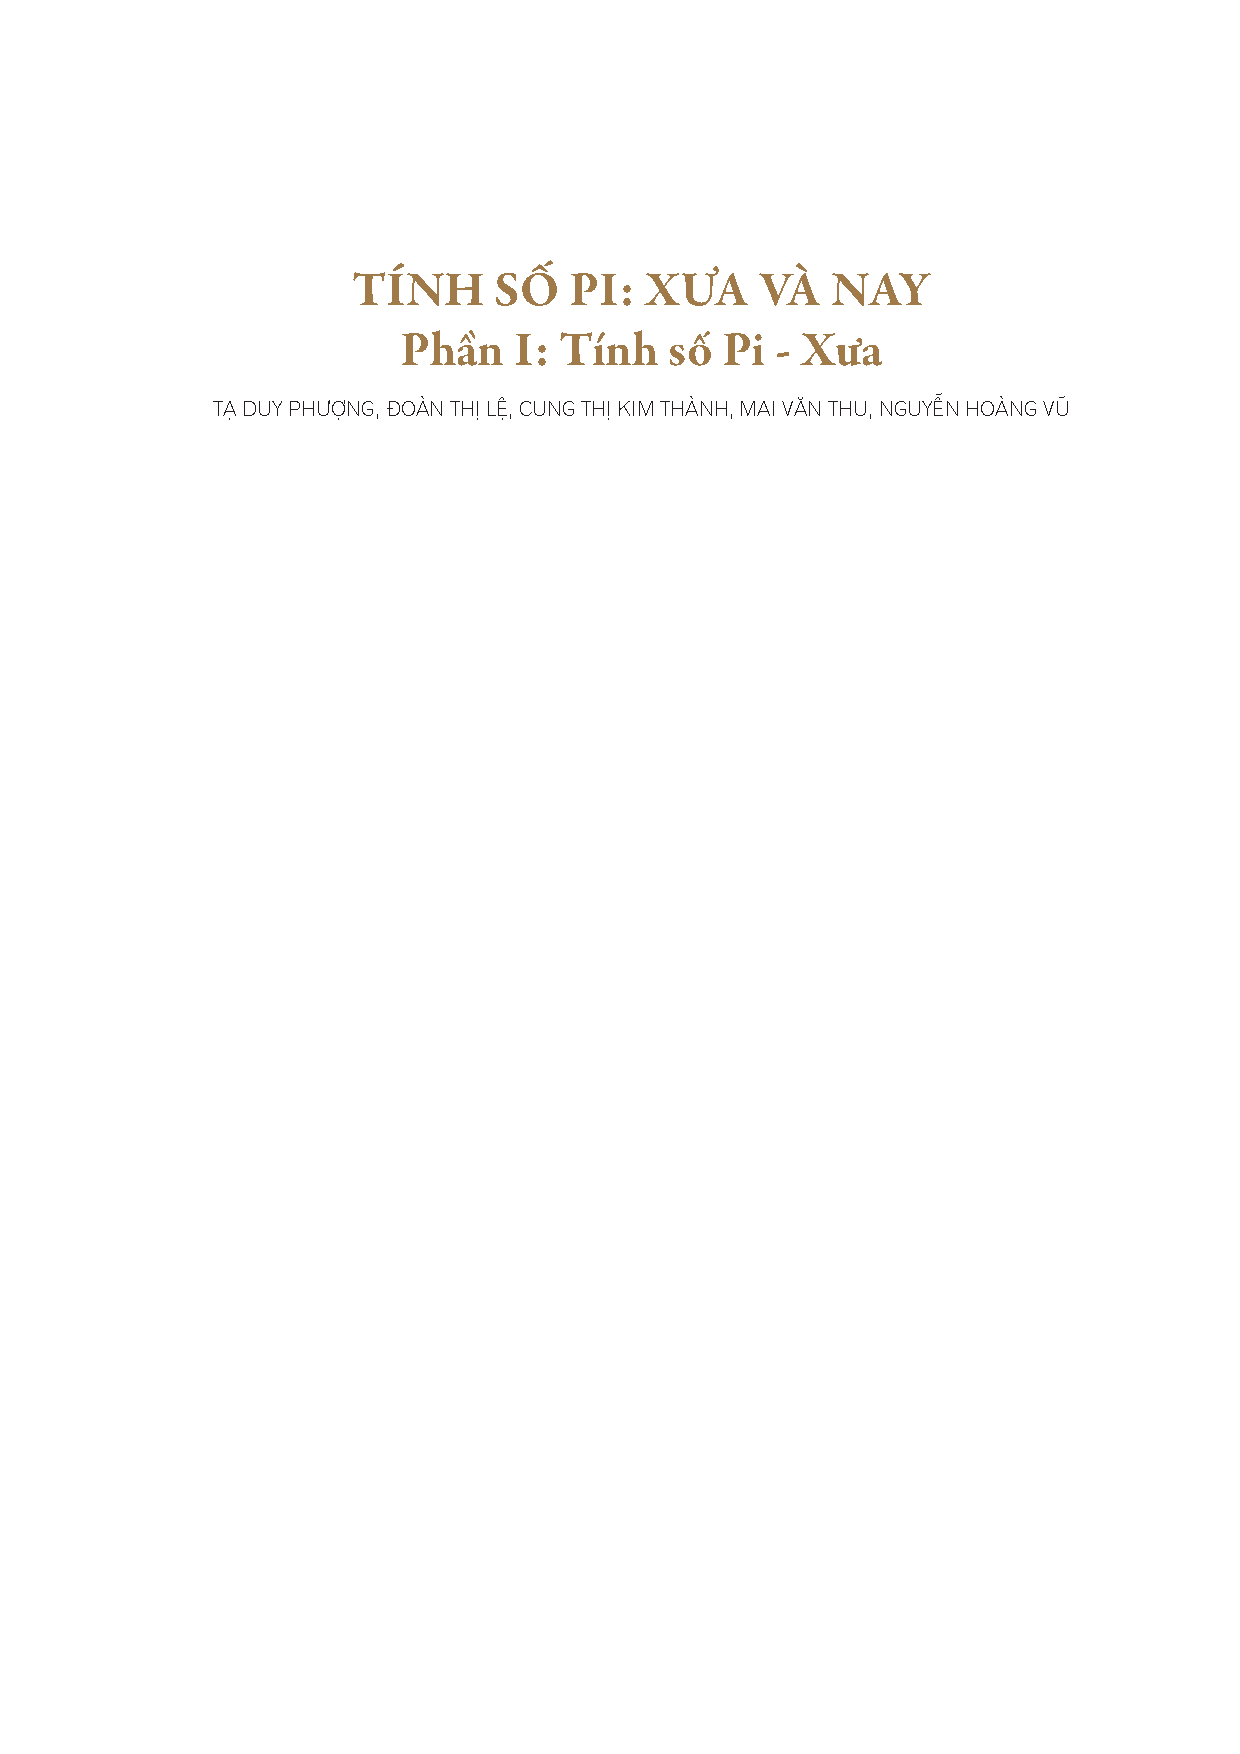
\includegraphics[scale=1]{../tieude.pdf}}}
\centering
\endgroup

\vspace*{185pt}

\begin{multicols}{2}
	\textbf{\color{lichsutoanhoc}Nhập đề.}
	Chúng ta có rất ít thông tin về cuộc đời các nhà toán học Hy Lạp vĩ đại. Euclid cũng không ngoại lệ. Tất cả những gì được biết về ông chứa trong một vài câu tóm tắt của Proclus: (Euclid, người đã viết \textit{Cơ sở} (\textit{Elements}), trong đó tập hợp nhiều định lý của Eudoxus, hoàn thiện nhiều kết quả của Theaetetus, đồng thời đã chứng minh rõ ràng, chặt chẽ và sắp xếp lại trong một trật tự logic rất nhiều kết quả chỉ được chứng minh một cách lỏng lẻo bởi những người đi trước.)
		\begin{figure}[H]
		\vspace*{-5pt}
		\centering
		\captionsetup{labelformat= empty, justification=centering}
		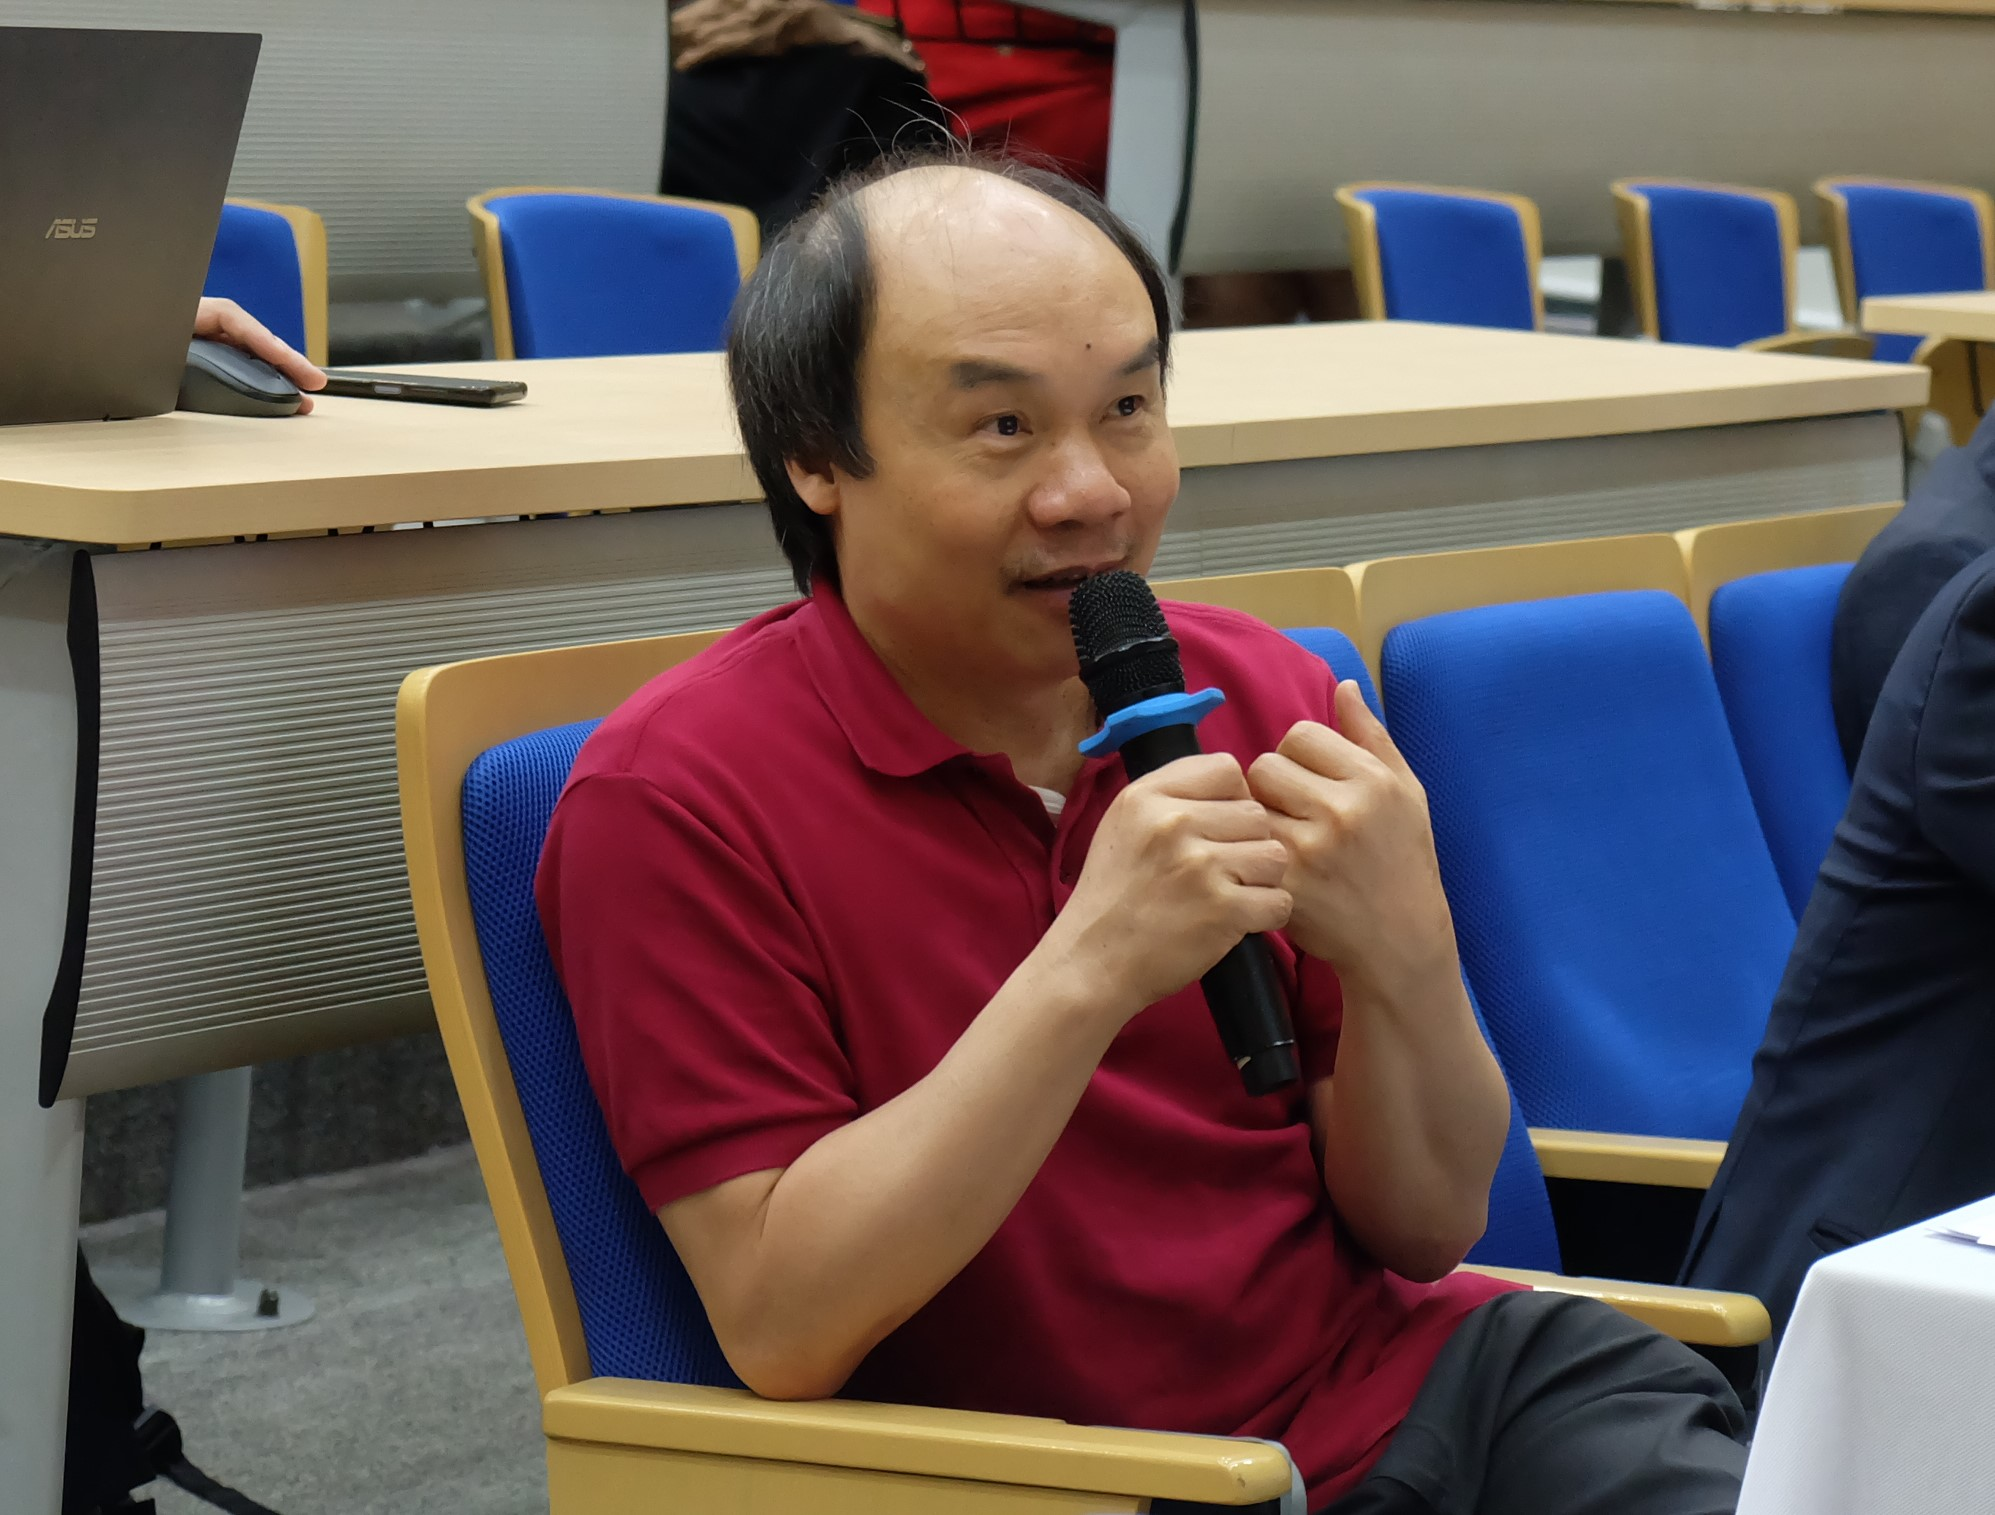
\includegraphics[width= 1\linewidth]{1}
		\vspace*{-10pt}
	\end{figure}
	Như vậy, ngay cả nhà triết học Proclus ($411-485$ Công nguyên, viết tắt: CN), người đã viết nhiều cuốn sách về triết học và toán học Hy Lạp, trong đó có cuốn sách bình luận về \textit{Cơ sở} của Euclid [$8$], cũng không cho biết chính xác năm sinh, năm mất và nơi sinh của Euclid. Proclus chỉ cho biết Euclid trẻ hơn các học trò đầu tiên của Plato, nhiều tuổi hơn Eratosthenes và Archimedes. Plato mất vào năm $347$ trước Công nguyên (viết tắt: TCN) và Archimedes sống trong khoảng năm $287$ đến $212$ TCN. Vì vậy, các nhà viết sử cho rằng Euclid sống vào khoảng những năm $300$ TCN, dưới thời Ptolemy I, người trị vì từ $306$ đến $283$ TCN và Ptolemy II ($309-246$ TCN, người trị vì từ $284$ đến $246$ TCN). 
	\vskip 0.1cm
	Phần đầu bài viết này giới thiệu nội dung cơ bản và những đánh giá về \textit{Cơ sở} và các tác phẩm khác của Euclid, chủ yếu dựa trên [$1$]. Các phần sau dựa trên sự tổng hợp của các tài liệu [$1$]--[$8$].
	\vskip 0.1cm
	\textbf{\color{lichsutoanhoc}Bối cảnh ra đời của Elements.}
	Alexander Đại đế đã chinh phục phần lớn thế giới trong vòng $12$ năm ($334-323$ TCN). Vì quân đội của ông chủ yếu là người Hy Lạp nên ông đã truyền bá văn hóa Hy Lạp sang một phần rộng lớn của vùng Cận Đông. Tiếp theo là một chương mới của lịch sử, được gọi là \textit{Thời đại Hy Lạp hóa} (Hellenistic) hoặc \textit{tựa Hy Lạp} (Greek--like), kéo dài trong ba thế kỷ, cho đến khi đế chế La Mã được thành lập.
	\vskip 0.1cm
	Sau khi Alexander qua đời, Ptolemy, một trong những vị tướng hàng đầu của Alexander, trở thành Thống đốc của Ai Cập và hoàn thành việc xây dựng thành phố Alexandria. Alexandria nhanh chóng tỏa sáng và làm lu mờ Athens, khiến Athens bị giảm xuống vị thế của một thành phố tỉnh lẻ. Trong gần $1000$ năm, Alexandria là trung tâm phát triển của văn hóa Hy Lạp hóa.
	\vskip 0.1cm
	Các thế hệ vua Ptolemy đã làm hết mình để biến Alexandria thành trung tâm của đời sống trí thức cho toàn bộ Địa Trung Hải. Họ đã xây dựng một trung tâm lớn của học thuật, gọi là \textit{Bảo tàng} (Musaeum), ở đây có nghĩa là \textit{Ngôi đền của các nàng thơ} (Temple of the Muses), tiền thân của trường đại học hiện đại. Các học giả hàng đầu của thời đại--các nhà khoa học, nhà thơ, nghệ sĩ và nhà văn--đã đến Alexandria theo lời mời của các vua Ptolemy với lòng hiếu khách đặc biệt. Các học giả có thể ở lại \textit{Bảo tàng} bao lâu tùy thích, Tại \textit{Bảo tàng}, họ có thời gian rảnh rỗi để theo đuổi việc nghiên cứu, tiếp cận các sách cổ trong thư viện và có cơ hội thảo luận các vấn đề với các chuyên gia.  Ngoài ăn ở miễn phí, họ được trả lương, với yêu cầu duy nhất là họ phải giảng bài. Các học giả sống trong \textit{Bảo tàng} với chi phí của nhà vua trong điều kiện sang trọng, với các phòng giảng rộng rãi và lộng lẫy, có thể đi dạo trong các hành lang với các hàng cột tráng lệ. Bảo tàng có một phòng ăn rộng lớn, nơi các học giả dùng bữa cùng nhau. 
	\vskip 0.1cm
	Được xây dựng như một tượng đài cho sự huy hoàng của dòng họ Ptolemy, \textit{Bảo tàng} đã là một cột mốc quan trọng trong lịch sử khoa học. Nó được xây dựng như là một tổ chức nghiên cứu và học thuật, hơn là một cơ quan giáo dục, cho các học giả và các nhà khoa học đến sống và làm việc tại đây hàng mấy thế kỷ. Ở đỉnh cao của nó, trung tâm này có đến vài trăm chuyên gia, sự hiện diện của họ đã thu hút nhiều thế hệ trẻ háo hức đến học tập và phát triển tài năng. Khoa học và toán học thời kỳ này đã phát triển với thành công đáng kể. Trong lịch sử toán học chỉ có một thời gian khác trong khoảng $200$ năm có thể so sánh với giai đoạn $300-100$ trước Công nguyên, đó là khoảng thời gian từ Kepler đến Gauss ($1600-1850$).
	\begin{figure}[H]
		\vspace*{-10pt}
		\centering
		\captionsetup{labelformat= empty, justification=centering}
		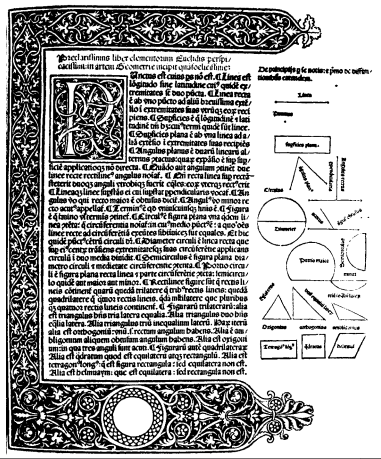
\includegraphics[width= 1\linewidth]{2}
		\caption{\small\textit{\color{lichsutoanhoc}Một trang từ cuốn sách Elements của Euclid in lần đầu tiên bằng tiếng Latin năm $1482$.}}
		\vspace*{-10pt}
	\end{figure} 
	Các học giả không thể sống mà không có sách, vì vậy nhu cầu đầu tiên là thu thập các bản thảo. Được thành lập gần như đồng thời với \textit{Bảo tàng} và liền kề với nó là \textit{Thư viện lớn} của Alexandria, nơi chứa bộ sưu tập lớn nhất các tác phẩm Hy Lạp còn tồn tại. Tất nhiên trước đó đã có những thư viện, nhưng không có thư viện nào sở hữu những tài nguyên lớn như thư viện Alexandria. Các bản thảo được tìm kiếm trên khắp thế giới và có những đại lý được ủy quyền để sao chép các tác phẩm nếu không mua được chúng. Du khách đến Alexandria được yêu cầu giao nộp bất kỳ cuốn sách nào chưa có trong thư viện.
	\vskip 0.1cm
	Trước khi Bảo tàng chìm vào quên lãng năm $641$, nó đã tạo ra nhiều tác phẩm nổi bật của các học giả, xác định tiến trình phát triển của toán học trong nhiều thế kỷ: Euclid, Archimedes, Apollonius, Ptolemy và Diophantus.
	\vskip 0.1cm
	Các nhà lịch sử thống nhất cho rằng, Euclid là một học giả tích cực của \textit{Bảo tàng} và \textit{Thư viện}, dưới triều đại Ptolemy I và II. 
	\vskip 0.1cm
	Hậu thế biết đến Euclid như là tác giả của \textit{Cơ sở của hình học} (\textit{Elements of Geometry}), một cuốn sách toán học quan trọng nhất của văn hóa Hy Lạp và có lẽ của tất cả các thời đại. \textit{Cơ sở} là tập hợp các kiến thức quan trọng nhất vào thời điểm đó, được sắp xếp thành $13$ phần, hay $13$ chương ($13$ quyển). Sáu quyển đầu dành cho hình học phẳng, ba quyển tiếp theo về số học. Quyển X cung cấp mối liên hệ giữa hai đại lượng: độ lớn (magnitude) được trình bày trong Quyển V và các con số (number) trong quyển VII. Quyển XI nghiên cứu hình học không gian và Quyển XII trình bày phương pháp vét cạn (method of exhaustion) cho cả hình phẳng và hình không gian. Và cuối cùng, Quyển XIII trình bày năm khối đa diện đều và phân loại các đường đã được trình bày trong Quyển X.   
	\vskip 0.1cm
	Mặc dù đã có một vài cuốn sách toán trước \textit{Cơ sở}, nhưng không quyển nào được bảo  tồn, vì lý do rõ ràng là tất cả đã bị lu mờ và được thay thế bởi cuốn sách của Euclid.
	\vskip 0.1cm
	Mặc dù phần lớn kết quả đã có từ trước, nhưng sự sắp xếp hợp lý đến tuyệt vời của các định lý và sự phát triển của các sự kiện cho thấy thiên tài của Euclid. Ông đã hợp nhất các khám phá biệt lập thành một hệ thống các định đề, định nghĩa và tiên đề ban đầu, để từ đó suy ra các kết quả (định lý) theo một thứ tự suy diễn duy nhất.
	\vskip 0.1cm
	Gần như không có cuốn sách nào quan trọng đối với tư tưởng và giáo dục của phương Tây hơn là \textit{Cơ sở} của Euclid. Hiếm có cuốn sách nào, ngoại trừ Kinh Thánh, đã được xuất bản, lưu hành và nghiên cứu rộng rãi như \textit{Cơ sở}. Trong suốt $2000$ năm, sáu cuốn sách đầu tiên của \textit{Cơ sở} là  sách giáo khoa hình học của học sinh. Hơn $1000$ phiên bản của \textit{Cơ sở} đã xuất hiện kể từ bản in đầu tiên bằng tiếng Latin ra đời năm $1482$. Và trước đó, các bản sao viết tay đã thống trị phần lớn việc giảng dạy toán học ở châu Âu.
	\begin{figure}[H]
		\vspace*{-5pt}
		\centering
		\captionsetup{labelformat= empty, justification=centering}
		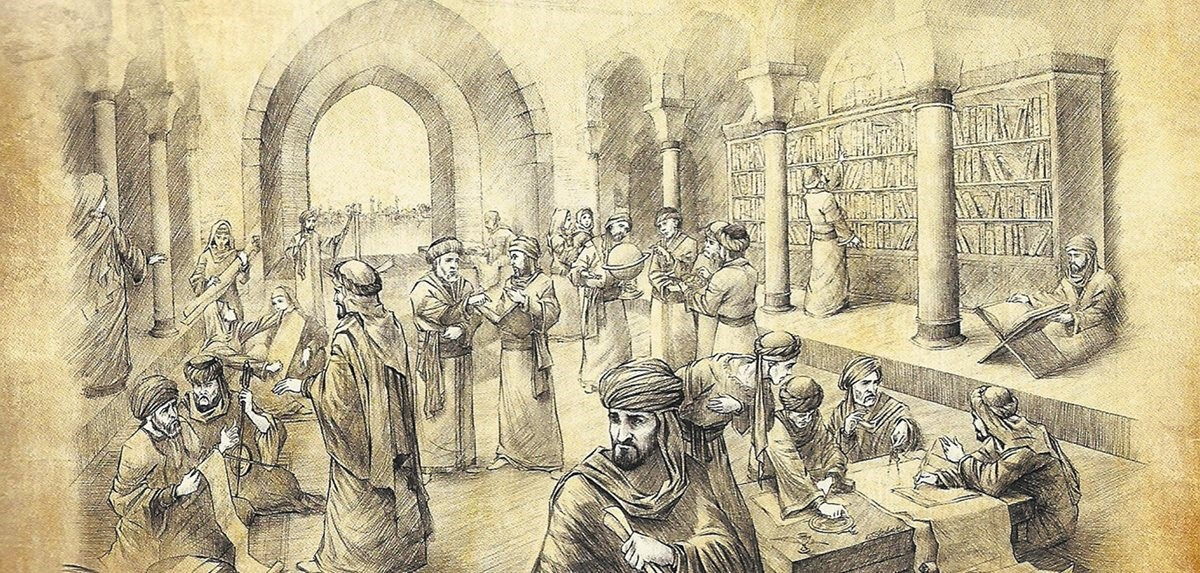
\includegraphics[width= 1\linewidth]{3}
		\caption{\small\textit{\color{lichsutoanhoc}Bìa trước của bản dịch tiếng Anh đầu tiên của Henry Billingsley năm $1570$.}}
		\vspace*{-10pt}
	\end{figure} 
	Mặc dù danh tiếng của Euclid, cả trong thời cổ đại và thời hiện đại, hầu như chỉ dựa vào \textit{Cơ sở}, nhưng ông còn là tác giả của ít nhất $10$ tác phẩm khác về nhiều chủ đề khác nhau. Văn bản tiếng Hy lạp cuốn \textit{Dữ liệu} (\textit{Data}), một tuyển tập gồm $95$ bài tập có lẽ dành cho những sinh viên đã hoàn thành \textit{Cơ sở}, là văn bản duy nhất khác của Euclid về hình học còn tồn tại. Một chuyên luận, \textit{Các thiết diện conic} (\textit{Conic Sections}), là nền tảng của bốn cuốn sách đầu tiên trong tác phẩm cùng tên của Apollonius, đã bị thất lạc. Và tác phẩm \textit{Các hệ quả} (\textit{Porisms}) cũng  chung số phận. Rõ ràng \textit{Các thiết diện conic} là một cuốn sách về hình học cao cấp, là một bản cổ xưa nhất của hình học giải tích. Ngoài ra, ông còn có \textit{Phân chia các  hình} (\textit{Division of Figures}), \textit{Hiện tượng} (\textit{Phaenomena}), và \textit{Quang học} (\textit{Optics}),...
	\vskip 0.1cm
	Chúng ta biết rất ít về cuộc sống cá nhân của Euclid.  Chỉ biết chắc chắn ông đã thành lập một trường học và giảng dạy ở Alexandria, nhưng không có gì khác được biết ngoại trừ điều đó. Có khả năng ông đã được đào tạo toán học ở Athens dưới sự dẫn dắt của các học trò của Plato. Hai giai thoại sau có thể là những minh chứng cho tính cách của Euclid. Giai thoại thứ nhất kể rằng, khi nhà vua Ptolemy I hỏi ông liệu có con đường nào ngắn để tiếp thu hình học hơn là \textit{Cơ sở} không, ông đã trả lời: ``Thưa Bệ hạ, không có con đường hoàng gia tới hình học" (``There is no royal road to Geometry"), ngụ ý là toán học bình đẳng với tất cả mọi người, Một câu chuyện khác, do Stobaeus (thế kỷ $5$) kể lại, liên quan đến một thanh niên bắt đầu học hình học với Euclid và hỏi, sau khi đã học các định lý đầu tiên: ``Nhưng tôi sẽ nhận được gì sau khi học những điều này?" Euclid đã gọi người hầu của mình đến và bảo rằng: ``Hãy cho người đàn ông này một đồng xu, vì anh ta phải kiếm được lợi nhuận từ những gì anh ta học được." Lời quở trách có lẽ đã được chuyển thể từ một câu châm ngôn của trường phái Pythagoras: ``Một sơ đồ và một bước (trong kiến thức), không phải là một sơ đồ và một đồng xu." (``A diagram and a step (in knowledge), not a diagram and a coin.")  
	Thiết nghĩ những câu chuyện này vẫn còn mang tính thời sự đến tận ngày nay.
	\vskip 0.1cm
	\textbf{\color{lichsutoanhoc}Cơ sở hình học của Euclid}
	\vskip 0.1cm
	Trong hơn hai nghìn năm, Euclid đã là người phát ngôn của hình học Hy Lạp, sự sáng tạo tuyệt vời nhất của trí tuệ Hy Lạp. Kể từ thời của ông, việc nghiên cứu \textit{Cơ sở} là điều cần thiết với một nền giáo dục khai phóng. Thế hệ này qua thế hệ khác đã coi \textit{Cơ sở} là đỉnh cao của logic, và nghiên cứu nó là cách tốt nhất làm cơ sở cho suy luận chính xác.  Chỉ trong vòng $100$ năm trở lại đây, \textit{Cơ sở} mới bắt đầu bị thay thế bởi các sách giáo khoa hiện đại. Tuy nhiên, tác phẩm của Euclid vẫn là mô hình tối cao về toán học thuần túy.
	\vskip 0.1cm
	Bất kỳ ai quen thuộc với quá trình thao tác trí tuệ đều nhận ra rằng nội dung của \textit{Cơ sở} không thể là nỗ lực của một cá nhân đơn lẻ. Có lẽ không nhiều các định lý được thiết lập trong \textit{Cơ sở} là do chính Euclid khám phá ra. Sự vĩ đại của Euclid nằm ở chỗ ông đã sắp xếp một khối lượng lớn các kiến thức độc lập của toán học Hy Lạp về hình học và lý thuyết số vào một trật tự logic chặt chẽ, có quan hệ mật thiết với nhau. Kết quả này tiếp nối kết quả khác với tối thiểu các giả thiết. Uy tín của \textit{Cơ sở} lớn đến mức tác giả của nó hiếm khi được gọi bằng tên mà bằng \textit{Tác giả của Elements} hoặc đơn giản là \textit{Nhà hình học}.
	\vskip 0.1cm 
	Euclid nhận thức được rằng để tránh vòng luẩn quẩn và cung cấp một điểm khởi đầu, một số sự kiện về bản chất của đối tượng phải được coi là một sự thật hiển nhiên mà không cần chứng minh, được gọi là các \textit{tiên đề}. Theo một nghĩa nào đó, chúng là những ``luật chơi" mà từ đó tất cả các suy luận có thể tiến hành, là nền tảng mà toàn bộ các định lý phải dựa vào.
	\vskip 0.1cm
	Euclid đã cố gắng xây dựng toàn bộ tòa nhà kiến thức hình học Hy Lạp, được tích lũy kể từ thời Thales, trên $5$ định đề có bản chất hình học cụ thể và $5$ tiên đề được dùng làm nền móng cho toàn bộ lâu đài toán học. Ba định đề đầu tiên là định đề xây dựng, khẳng định những gì chúng ta được phép vẽ. Từ đó, ông suy ra từ $10$ giả định này $465$ mệnh đề qua một chuỗi suy luận logic, sử dụng chúng như những viên đá lót đường trong một cuộc diễu hành có trật tự từ một mệnh đề đã được chứng minh sang một mệnh đề khác. Điều kỳ diệu là rất nhiều mệnh đề thú vị có thể thu được chỉ từ một vài tiên đề được lựa chọn một cách  khôn ngoan. 
	\vskip 0.1cm
	Đột ngột và không có bình luận giới thiệu, cuốn sách đầu tiên của \textit{Cơ sở} mở ra với danh sách $23$ định nghĩa (xem [$2b$], trang $16-18$). Chúng bao gồm, thí dụ, điểm là gì, đường là gì (Định nghĩa $1$, $2$) và kết thúc bằng Định nghĩa $23$: ``Các đường thẳng song song là các đường thẳng cùng nằm trong một mặt phẳng và khi kéo dài đến vô tận ở cả hai hướng thì không gặp nhau ở cả hai hướng." Các định nghĩa này không được coi là định nghĩa theo nghĩa hiện đại. Mặc dù mơ hồ và không hữu ích trong một số khía cạnh, chúng cũng đủ để tạo ra một số hình ảnh trực quan nhất định. Một số thuật ngữ kỹ thuật được sử dụng, thí dụ chu vi đường tròn, hoàn toàn không được định nghĩa. Thật lạ lùng khi Euclid đã định nghĩa đường thẳng song song, lại không đưa ra một định nghĩa chính thức về hình bình hành.
	\vskip 0.1cm
	Sau các định nghĩa, Euclid đặt ra $10$ nguyên tắc mà chứng minh các mệnh đề và định lý phải dựa trên. Đó là (xem thêm [$2b$], trang $19-20$):
	\vskip 0.1cm
	\textbf{\color{lichsutoanhoc}Các định đề:}
	\vskip 0.1cm
	$1.$ Cùng quy ước rằng có thể vẽ một đoạn thẳng nối hai điểm bất kì.
	\vskip 0.1cm
	$2.$ Và có thể kéo dài liên tục một đoạn thẳng thành đường thẳng.
	\vskip 0.1cm
	$3.$ Có thể vẽ một đường tròn có tâm và bán kính bất kì.
	\vskip 0.1cm
	$4.$ Tất cả các góc vuông đều bằng nhau.
	\vskip 0.1cm
	$5.$ Nếu một đường thẳng cắt hai đường thẳng khác tạo thành các góc trong về cùng một phía [với nó] có tổng nhỏ hơn $2$ góc vuông, thì hai đường thẳng (bị cắt) khi kéo dài ra vô tận sẽ cắt nhau ở phía của đường thẳng ban đầu mà tổng các góc trong nhỏ hơn $2$ vuông (chứ không cắt ở phía bên kia). 
	\vskip 0.1cm
	\textbf{\color{lichsutoanhoc}Các tiên đề:}
	\vskip 0.1cm
	$1.$ Những thứ cùng bằng một thứ thì bằng nhau.
	\vskip 0.1cm
	$2.$ Nếu cùng thêm những thứ bằng nhau vào những thứ bằng nhau thì những tổng sẽ bằng nhau.
	\vskip 0.1cm
	$3.$ Nếu cùng bớt những thứ bằng nhau vào những thứ bằng nhau thì những phần còn lại sẽ bằng nhau.
	\vskip 0.1cm
	$4.$ Các thứ trùng nhau thì bằng nhau.
	\vskip 0.1cm
	$5.$ Tổng thể thì lớn hơn bộ phận.
	\vskip 0.1cm
	Định đề $5$, còn gọi là \textit{Định đề song song}, đã trở thành một trong những phát biểu nổi tiếng và gây tranh cãi nhất trong lịch sử toán học. Thậm chí có ý kiến cho rằng Euclid không hoàn toàn hài lòng với Định đề $5$. Ông đã trì hoãn sử dụng của nó cho đến khi không thế tiến xa hơn nếu không có nó, mặc dù việc sử dụng nó sớm hơn sẽ đơn giản hóa nhiều chứng minh các định lý.
	\vskip 0.1cm
	Hơn $2000$ năm, từ lúc xuất hiện \textit{Cơ sở} đến thế kỷ $19$, các nhà toán học đã cố gắng rút ra định đề song song từ bốn định đề đầu tiên, tin rằng bốn định đề này cùng với $5$ tiên đề là đủ cho sự phát triển hoàn chỉnh hình học Euclid. Tất cả những nỗ lực nhằm thay đổi trạng thái từ ``Định đề $5$" thành định lý" đều thất bại, vì mỗi nỗ lực đều dựa trên giả định ẩn tương đương với chính định đề đó. 
	\vskip 0.1cm
	Tuy nhiên, những nỗ lực này đã dẫn đến việc phát hiện ra hình học phi--Euclid, trong đó các Định đề của Euclid, ngoại trừ định đề song song đều đúng và các định lý của Euclid đều đúng, ngoại trừ những định lý dựa trên định đề song song. Thiên tài của Euclid thể hiện ở chỗ ông đã nhận ra rằng Định đề $5$ đòi hỏi tuyên bố rõ ràng như một giả định, không thể được chứng minh.   
	\vskip 0.1cm
	Khi xem xét Định đề $5$ Euclid, nhà toán học Giovanni Saccheri $(1667-1733)$ đã phân loại:
	\vskip 0.1cm
	Trường hợp $1$: Qua điểm đã cho có duy nhất đường thẳng song song với đường thẳng đã cho.
	\vskip 0.1cm
	Trường hợp $2$: Qua điểm đã cho có nhiều hơn một đường thẳng song song với đường thẳng đã cho.
	\vskip 0.1cm
	Trường hợp $3$: Qua điểm đã cho không có đường thẳng nào song song với đường thẳng đã cho.
	\vskip 0.1cm
	Trường hợp $1$ cho ta hình học Euclid, Trường hợp $2$ dẫn đến hình học Lobachevsky, Trường hợp $3$ cho ta hình học Riemann.
	\vskip 0.1cm
	Việc xem xét kĩ lưỡng trong hơn $2000$ năm đã phát lộ nhiều điểm sáng và những nhược điểm trong cách xử lý hình học của Euclid. Hầu hết các định nghĩa của ông đều dễ bị chỉ trích trên cơ sở này hay cơ sở khác. Xét cho cùng, một định nghĩa chỉ mang lại ý nghĩa của một từ theo nghĩa khác, đơn giản hơn--hoặc những từ mà ý nghĩa của nó đã rõ ràng. Những từ này đến lượt chúng lại được định nghĩa bằng những từ thậm chí còn đơn giản hơn. Rõ ràng quá trình định nghĩa như vậy phải có kết thúc. Cách duy nhất để tránh một vòng tròn luẩn quẩn là cho phép một số khái niệm ban đầu không được định nghĩa.
	Euclid đã nhầm khi cố gắng giải nghĩa toàn bộ từ vựng mà ông đã sử dụng. Chắc chắn điều này dẫn tới một số định nghĩa kỳ lạ và không thỏa đáng. Thí dụ: ``Điểm là cái không thể chia nhỏ", ``Đường không có chiều rộng". Vậy ``chia nhỏ" và ``chiều rộng" là gì? Ý tưởng về ``điểm" và ``đường thẳng" là những khái niệm cơ bản nhất trong hình học, chúng có thể được mô tả và được giải thích nhưng không thể được định nghĩa thỏa đáng bằng các định nghĩa đơn giản hơn chính chúng. Phải có một sự khởi đầu ở đâu đó trong một hệ thống khép kín, vì vậy chúng nên được chấp nhận không có định nghĩa.
	\vskip 0.1cm
	Có lẽ sự phản đối lớn nhất đã được đưa ra chống lại tác giả \textit{Cơ sở} là sự bất cập đáng tiếc trong các tiên đề của ông. Ngoài những thiếu sót hiển nhiên như  không nêu được sự tồn tại của điểm và đường thẳng hoặc đường thẳng nối hai điểm là duy nhất, Euclid đã đưa ra một số giả định ngầm được sử dụng sau này trong các chứng minh nhưng không xuất phát từ các định đề. Khá nhiều chứng minh của Euclid dựa trên hình vẽ và bằng chứng trực quan. Điều này được minh họa bằng lập luận được sử dụng ngay trong mệnh đề đầu tiên dưới đây trong \textit{Cơ sở}.
	\vskip 0.1cm 
	\textbf{\color{lichsutoanhoc}Mệnh đề} $\pmb{1}$ Cho một đoạn $AB$. Tồn tại tam giác đều có đoạn thẳng là một trong các cạnh của nó.
	\vskip 0.1cm
	\textbf{\color{lichsutoanhoc}Chứng minh} Sử dụng Định đề $3$, vẽ đường tròn tâm $A$ bán kính $AB$ đi qua điểm $B$. Từ tâm $B$ vẽ đường tròn bán kính $BA$ đi qua $A$. Từ giao điểm $C$ của hai đường tròn, dựng đoạn thẳng $CA$ và $CB$ (Định đề $1$).  Ta thấy $AC=AB$ và $BC=AB$ vì chúng là các bán kính của một đường tròn. Từ Tiên đề $1$ suy ra $AC=AB=BC$. Vậy các đoạn thẳng $AB, AC, BC$ tạo thành tam giác đều có đoạn thẳng $AB$ cho trước là một cạnh.
	\vskip 0.1cm
	\textbf{\color{lichsutoanhoc}Lời bình.} Ở đây có một vấn đề: Trên cơ sở trực giác, ta thấy hai đường tròn tâm $A$ và tâm $B$ chắc chắn cắt nhau tại $C$.  Tuy nhiên, mục đích của một lý thuyết tiên đề chính xác là phải cung cấp một hệ thống lý luận không phụ thuộc vào trực giác. Toàn bộ chứng minh sẽ đổ bể nếu các đường tròn ta xây dựng là không cắt nhau. Và điều này (đường tròn cắt nhau) không thể suy ra từ các định đề và tiên đề. Để khắc phục tình trạng này, phải bổ sung thêm một định đề đảm bảo tính ``liên tục" của các đường thẳng và đường tròn. Các nhà toán học sau này đã phải bổ sung thêm:
	\vskip 0.1cm
	\textit{Nếu một đường tròn hoặc đường thẳng có một điểm ở ngoài và một điểm ở trong một đường tròn khác thì nó có hai điểm chung với đường tròn.}
	\vskip 0.1cm 
	Phát biểu đơn thuần của định đề liên quan đến các khái niệm ``bên trong" và ``bên ngoài" không xuất hiện rõ ràng trong \textit{Cơ sở}. Nếu hình học muốn phát huy hết danh tiếng của nó về tính chặt chẽ logic hoàn hảo, thì nó phải chú ý đáng kể đến ý nghĩa của các thuật ngữ đó và các tiên đề chi phối chúng. 
	\vskip 0.1cm
	Trong suốt $25$ năm cuối của thế kỷ $19$, nhiều nhà toán học đã cố gắng xây dựng một hệ tiên đề đầy đủ và cần thiết để chứng minh tất cả các định lý quen thuộc từ lâu trong hình học Euclid. Nghĩa là, họ đã cố gắng bổ sung thêm những định đề nhằm mang lại tính rõ ràng và chặt chẽ cho những ý tưởng mà Euclid đã nhận ra bằng trực giác.  Người thành công nhất trong lĩnh vực này là David Hilbert ($1862-2943$) với tác phẩm \textit{Cơ sở Hình học} in năm $1899$ [$9$] (Grundlagen der Geometrie, tiếng Anh: \textit{Foundations of Geometry}). Trong tác phẩm này, Hilbert đã xây dựng lại hình học Euclid dựa trên năm nhóm tiên đề: các tiên đề về tính liên thông, các tiên đề về thứ tự, Tiên đề về song song (Tiên đề Euclid), các tiên đề về đồng dạng và Tiên đề về liên tục.  Hệ tiên đề này phải bảo đảm tính \textit{đơn giản}, tính \textit{đầy đủ} và tính \textit{độc lập}, khiến hình học Euclid trở nên hoàn hảo hơn.  
	\vskip 0.1cm
	\textbf{\color{lichsutoanhoc}Lý thuyết số của Euclid}
	\vskip 0.1cm
	\textbf{\color{lichsutoanhoc}Các tính chất chia hết.} Mặc dù công trình vĩ đại của Euclid có tựa đề \textit{Cơ sở của Hình học}, chủ đề của nó mở rộng vượt xa những gì chúng ta bây giờ coi là hình học phổ thông. Quyển II và Quyển V hầu như chỉ có đại số (đại số hình học). Ba quyển VII, VIII, IX chứa tổng cộng $102$ mệnh đề, được dành cho \textit{số học Hy Lạp}, nghĩa là số học trên tập các số tự nhiên (với sự mở rộng chứng minh $\sqrt{2}$ là số vô tỷ,...). Euclid đã viết các chương này chủ yếu dựa trên nội dung những cuốn sách số học có thể bắt nguồn từ trường phái Pythagoras. Tuy nhiên, ông đã sắp xếp toàn bộ các kiến thức đã có trong một trật tự hợp lý. Nhiều kết quả đã biết từ trước nhưng không phải cái nào cũng được chứng minh một cách chặt chẽ. Nhiều công trình về lý thuyết số được viết trước có thể đã không còn tồn tại. Vì vậy, không thể phân biệt được cái nào là đã có từ trước và cái nào là do Euclid khám phá. 
	\vskip 0.1cm
	Quyển VII mở đầu với danh sách $22$ định nghĩa phân biệt các số khác nhau: số lẻ và số chẵn, số nguyên tố và hợp số, số hoàn hảo (là số bằng tổng các ước của nó, không tính chính nó).... Các định lý trong Quyển VII, VIII và IX là quen thuộc với học sinh phổ thông, nhưng ngôn ngữ chứng minh thì không quen thuộc. Xuyên suốt ba quyển sách này, mỗi số được thể hiện bằng một đoạn thẳng, do đó mỗi số được Euclid gọi là số $AB$. Mọi đoạn thẳng (độ dài bằng số vô tỷ) có thể không biểu diễn được dưới dạng số hữu tỷ, nhưng mọi số hữu tỷ đều được biểu diễn bằng các đoạn thẳng.
	\vskip 0.1cm
	Do đó, Euclid không sử dụng cụm từ ``là bội số của" hay ``là thừa số của", mà Ông thay thế bằng ``được đo bằng" và ``đo" tương ứng. Nghĩa là, một số $n$  được đo bằng một số $m$  khác nếu có số thứ ba $k$  sao cho  $n = km$.
	\vskip 0.1cm
	Quyển VII bắt đầu bằng hai mệnh đề mà ngày nay được gọi là ``Thuật toán Euclid" tìm ước số chung lớn nhất (số đo) của hai số tự nhiên.
	\vskip 0.1cm
	Từ các mệnh đề đã được chứng minh, ta tìm được các định lý tương tự trong số học. Mệnh đề $8$ phát biểu rằng, $a = \frac{m}{n} b$ và $c = \frac{m}{n} d$ thì $a - c = \frac{m}{n} (b - d)$.  Mệnh đề VII.$24$ nói rằng, nếu $a$ và $b$  nguyên tố cùng nhau với $c$,  thì  $ab$ nguyên tố cùng nhau với $c$.  Quyển VII kết thúc bằng Mệnh đề VII.$39$ với quy tắc tìm bội số chung nhỏ nhất của các số.
	\vskip 0.1cm
	Quyển VIII là quyển ít kết quả nhất trong số $13$ cuốn của \textit{Cơ sở}. Nó bắt đầu với các mệnh đề về cấp số nhân (Euclid gọi là \textit{tỷ số liên tục}) và chuyển sang một số tính chất đơn giản của hình vuông và hình lập phương và kết thúc với Mệnh đề VIII.$27$: Nếu ta có một số ``không gian" (solid number) dạng $ma \cdot mb \cdot mc$  và một số không gian đồng dạng  $na \cdot nb \cdot nc$ thì tỷ số của chúng sẽ là  $m^3 : n^3$ ,tức là như một khối lập phương đối với một khối lập phương.
	\vskip 0.1cm
	Quyển IX, quyển cuối cùng trong ba quyển sách về lý thuyết số, chứa nhiều định lý quan trọng. Trong số đó nổi tiếng nhất là Mệnh đề IX.$20$ về sự tồn tại vô hạn số nguyên tố với chứng minh đơn giản bằng phản chứng: Giả sử tồn tại hữu hạn số nguyên tố. Gọi $P$ là tích của tất cả các số nguyên tố. Xét $N = P + 1$.  Khi ấy theo giả thiết $N$  không thể là số nguyên tố, hay $N$  phải là hợp số. Do đó nó phải chia hết cho $p$  là một trong các số nguyên tố. Nhưng $N$  chia cho bất kỳ số nguyên tố $p$  nào trong tích  $P$ cũng có số dư bằng $1$. Điều vô lý này dẫn đến điều giả sử có hữu hạn số nguyên tố là sai. Vậy có vô hạn số nguyên tố.
	\vskip 0.1cm
	Mệnh đề IX.$14$ chính là định lý mà ngày nay ta gọi là Định lý cơ bản của số học: \textit{Bất kỳ số tự nhiên nào lớn hơn $1$ cũng đều có thể biểu diễn được duy nhất dưới dạng tích của các số nguyên tố.}
	\vskip 0.1cm
	Mệnh đề IX.$35$ là một mệnh đề thú vị, vì nó cho một phương pháp, rất tao nhã, tính tổng các số hạng của cấp số nhân như sau: Từ
	\begin{align*}
		\frac{a_{n+1}}{a_n} = \frac{a_n}{a_{n-1}} = \ldots= \frac{a_2}{a_1},
	\end{align*}
	theo tính chất của tỷ lệ thức (Quyển VII), suy ra
	\begin{align*}
		\frac{a_{n+1} - a_n}{a_n} &= \frac{a_n - a_{n-1}}{a_{n-1}} = \ldots = \frac{a_3 - a_2}{a_2} \\
		&= \frac{a_2 - a_1}{a_1}.		
	\end{align*}
	Cộng tử với tử, mẫu với mẫu của tỷ lệ thức, ta có
	\begin{align*}
		\frac{a_{n+1} - a_1}{a_n + a_{n-1} + \ldots + a_1} = \frac{a_2 - a_1}{a_1}		
	\end{align*}
	Vậy  $S_n = \dfrac{a(1-r^n)}{1 -r}$,
	\vskip 0.1cm 
	trong đó $a = a_1$  là số hạng đầu tiên của cấp số nhân, $S_n = a_1 + \ldots + a_n$  là tổng của $n$  số hạng đầu của cấp số nhân và  $r = \frac{a_2}{a_1}$ là tỷ lệ (công bội).
	\vskip 0.1cm  
	Mệnh đề tiếp theo, cũng là mệnh đề cuối cùng trong Quyển IX nói về số hoàn hảo: Nếu  $S_n = 1 + 2 + 2^2 + \ldots + 2^{n-1} = 2^n -1$ là số hoàn hảo, thì  $2^{n-1}\left(2^n - 1\right)$ cũng là số hoàn hảo. Điều này có thể được chứng minh dễ dàng theo định nghĩa số hoàn hảo trong Quyển VII. Người Hy Lạp đã biết bốn số hoàn hảo: $6$, $28$, $496$ và $8128$.  Euclid không trả lời câu hỏi ngược lại: Công thức trên có cung cấp tất cả các số hoàn hảo không. Euler đã chứng minh rằng mọi số hoàn hảo chẵn đều có dạng trên, nhưng câu hỏi về sự tồn tại số hoàn hảo lẻ vẫn chưa có lời giải. Hiện nay người ta mới chỉ biết $39$ số hoàn hảo (chẵn).
	\vskip 0.1cm
	\textbf{\color{lichsutoanhoc}Tính vô ước của các đoạn thẳng (sự tồn tại số vô tỷ)}. Quyển X của tập \textit{Cơ sở}, trước khi đại số hiện đại ra đời, là tác phẩm được ngưỡng mộ nhất và cũng là đáng sợ nhất. Nó chứng minh sự tồn tại của số vô tỷ và liên quan đến sự phân loại có hệ thống của các đoạn không thông ước (hai đoạn thẳng có độ dài $a$  và $b$  được gọi là thông ước nếu tồn tại đoạn thẳng $k$  có độ dài hữu tỷ sao cho  $a = kb$). Cạnh của hình vuông và đường chéo của nó là không thông ước với nhau. Điều này có thể dễ dàng suy ra từ Định lý Pythagoras (xem [$10$], Tập $6$, số $5$: Chứng minh $\sqrt{2}$ là số vô tỷ).
	\vskip 0.1cm
	\textbf{\color{lichsutoanhoc}Hình học không gian}. Quyển XI gồm $39$ mệnh đề về các tính chất của các hình đa diện. Quyển XII liên quan đến đo lường (độ dài, diện tích, thể tích)  nhờ phương pháp vét cạn và áp dụng đo thể tích của kim tự tháp, hình nón, hình trụ và hình cầu. Archimedes đã gán các kết quả này cho Eudoxus, người mà có lẽ Euclid đã dựa vào để viết các quyển này.  Quyển XIII dành cho nghiên cứu $5$ khối đa diện đều.   
	\vskip 0.1cm
	\textbf{\color{lichsutoanhoc}Kết luận.} Trong một bài viết, không thể nói đầy đủ về \textit{Cơ sở} và các tác phẩm khác của Euclid. Bạn đọc muốn nghiên cứu \textit{Cơ sở} của Euclid với các phân tích sâu hơn, có thể đọc bản dịch tiếng Việt [$2b$] và các tài liệu tiếng Anh trong \textit{Tài liệu tham khảo}. Để phần nào thấy được toán học Hy Lạp đã được Euclid thể hiện trong \textit{Cơ sở} với một trật tự logic hoàn hảo như thế nào, bạn đọc có thể xem thêm [$10$] và các tài liệu trích dẫn trong đó. 
	\vskip 0.1cm
	\textbf{\color{lichsutoanhoc}Tài liệu tham khảo chính}
	\vskip 0.1cm
	[$1$] David M. Burton, T\textit{he History of Mathematics, An Introduction}, Seventh Edition, McGraw--Hill, $2011$. Ch. $4$: The Alexandrian School: Euclid, pp. $141-183$.
	\vskip 0.1cm
	[$2a$] Euclid's \textit{Elements of Geometry}, English translation from the Greek text of J.L. Heiberg ($1883-1885$): Richard Fitzpatrick, $2008$, $545$ p.
	\vskip 0.1cm
	[$2b$] Euclid, \textit{Cơ sở của Hình học}, Nhà xuất bản Trí thức, $2016$, $350$ trang.
	\vskip 0.1cm
	[$3$] Uta C. Merzbach and Carl B. Boyer, \textit{A
	History of Mathematics}, $3$th Edition, John Wiley \& Sons, $2011$, Ch. $5$: \textit{Euclid of Alexandria}, pp. $90-108$.
	\vskip 0.1cm
	[$4$] Thomas Heath, \textit{The thirteen books of Euclid’s Elements}, Translated from the text of Heiberg with introduction and commentary T. L. Heath, the University Press, Cambridge, $1908$.
	\vskip 0.1cm   
	\textbf{\color{lichsutoanhoc}Tài liệu tham khảo}
	\vskip 0.1cm
	[$5$] Thomas Heath, \textit{A History of Greek Mathematics}, Oxford at the Clarendon Press, $1921$, Volume $1$: \textit{Euclid}, pp. $354-446$.
	\vskip 0.1cm   
	[$6$] Stephen Hawking, \textit{God Created the Integers}, The mathematical Breakthroughs that changed History, Running Press, Euclid, pp. $1-118$.   
	\vskip 0.1cm
	[$7$] Victor J. Katz, \textit{A History of Mathematics, An Introduction}, Third Edition, Addison--Wesley, $2008$. Chapter $3$: Euclid, pp. $50-93$.
	\vskip 0.1cm
	[$8$] Proclus, \textit{The Philosophical and Mathematical Commentaries of Proclus}, Translated from the Greek by Thomas Taylor, London, $1792$.
	\vskip 0.1cm
	\textbf{\color{lichsutoanhoc}Tài liệu trích dẫn}
	\vskip 0.1cm
	[$9$] David Hilbert, \textit{Grundlagen der Geometrie}, $1899$. \textit{Foundations of Geometry}, Translation by E. J. Townsend, The Open Court Publishing Company, $1950$.
	\vskip 0.1cm
	[$10$] Tạ Duy Phượng, Các nhà toán học Hy Lạp. Tạp chí Pi, Tập $6$, số $4$, trang $46-50$; Tập $6$, số $5$, trang $45-53$, số $9$, trang $44-51$, số $10$, trang $56-59$; số $11$, trang $51-55$; Tập $7$, số $4$, trang $54-60$.
\end{multicols}